\documentclass[11pt]{article}
\usepackage[margin=1in]{geometry}
\usepackage[T1]{fontenc}
\usepackage{lmodern}
\usepackage{microtype}
\usepackage{amsmath,amssymb}
\usepackage{booktabs}
\usepackage{caption}
\captionsetup[table]{position=top,skip=6pt}
\usepackage{graphicx}
\usepackage{xcolor}
\usepackage{tikz}
\usetikzlibrary{arrows.meta,positioning,decorations.pathreplacing}
\usepackage[numbers,sort&compress]{natbib}
\usepackage[colorlinks=true,linkcolor=black,citecolor=blue!50!black,urlcolor=blue!50!black]{hyperref}
\usepackage{url}

% Generated by experiments/paper_assets.py from results/*.json. Do not edit.
\newcommand{\nAnnouncements}{1200}
\newcommand{\nUsable}{1148}
\newcommand{\nEvents}{1138}
\newcommand{\nTickers}{30}
\newcommand{\nNoDocWindow}{51}
\newcommand{\nAMC}{684}
\newcommand{\nBMO}{448}
\newcommand{\nDMH}{6}
\newcommand{\tokMedian}{6{,}862}
\newcommand{\tokPten}{2{,}999}
\newcommand{\tokPninety}{12{,}421}
\newcommand{\shareOverEight}{89}
\newcommand{\shareEncodedEight}{45}
\newcommand{\charMedian}{28{,}876}
\newcommand{\nExhibitStd}{1131}
\newcommand{\nHeadlineEvents}{111}
\newcommand{\firstHeadlineEntry}{2025-11-05}
\newcommand{\nTrain}{740}
\newcommand{\upTrain}{0.470}
\newcommand{\firstTrain}{2016-10-19}
\newcommand{\lastTrain}{2023-04-24}
\newcommand{\nVal}{169}
\newcommand{\upVal}{0.527}
\newcommand{\firstVal}{2023-04-27}
\newcommand{\lastVal}{2024-10-24}
\newcommand{\nTest}{229}
\newcommand{\upTest}{0.454}
\newcommand{\firstTest}{2024-10-31}
\newcommand{\lastTest}{2026-10-23}
\newcommand{\purgedTrain}{6}
\newcommand{\purgedVal}{4}
\newcommand{\selLRChunks}{1}
\newcommand{\selLRC}{0.01}
\newcommand{\selHeadChunks}{1}
\newcommand{\selHeadLayers}{0}
\newcommand{\nWeeks}{79}
\newcommand{\nBoot}{2{,}000}
\newcommand{\valMaj}{0.500}
\newcommand{\testMaj}{0.500}
\newcommand{\loMaj}{0.500}
\newcommand{\hiMaj}{0.500}
\newcommand{\valTick}{0.566}
\newcommand{\testTick}{0.487}
\newcommand{\loTick}{0.423}
\newcommand{\hiTick}{0.556}
\newcommand{\valLR}{0.539}
\newcommand{\testLR}{0.461}
\newcommand{\loLR}{0.383}
\newcommand{\hiLR}{0.538}
\newcommand{\valHead}{0.601}
\newcommand{\testHead}{0.506}
\newcommand{\loHead}{0.439}
\newcommand{\hiHead}{0.573}
\newcommand{\valZs}{0.532}
\newcommand{\testZs}{0.469}
\newcommand{\loZs}{0.388}
\newcommand{\hiZs}{0.552}
\newcommand{\valHeadSelect}{0.602}
\newcommand{\headSeedMin}{0.497}
\newcommand{\headSeedMax}{0.516}
\newcommand{\diffHeadTick}{$+$0.019}
\newcommand{\diffHeadTickLo}{$-$0.052}
\newcommand{\diffHeadTickHi}{$+$0.089}
\newcommand{\diffHeadLR}{$+$0.045}
\newcommand{\diffHeadLRLo}{$-$0.042}
\newcommand{\diffHeadLRHi}{$+$0.129}
\newcommand{\brierMaj}{0.248}
\newcommand{\loglossMaj}{0.689}
\newcommand{\brierHead}{0.259}
\newcommand{\loglossHead}{0.711}
\newcommand{\halfWidthHead}{0.067}
\newcommand{\explN}{111}
\newcommand{\explWeeks}{39}
\newcommand{\explAuc}{0.429}
\newcommand{\explLo}{0.323}
\newcommand{\explHi}{0.556}
\newcommand{\explBothN}{109}
\newcommand{\explDocAuc}{0.413}
\newcommand{\explDiff}{$+$0.022}
\newcommand{\explDiffLo}{$-$0.127}
\newcommand{\explDiffHi}{$+$0.182}
\newcommand{\negMean}{0.465}
\newcommand{\negSd}{0.075}
\newcommand{\negMin}{0.392}
\newcommand{\negMax}{0.578}
\newcommand{\posMean}{1.000}
\newcommand{\ctlRuns}{5}
\newcommand{\ctlTestN}{79}


\title{A Reproducible Financial NLP Pipeline for Post-Earnings Direction Classification:\\
A Pre-Registered Null Result on SEC Earnings Press Releases}
\author{Zackary Holt}
\date{October 2026}

\begin{document}
\maketitle

\begin{abstract}
We ask whether the language of a company's earnings press release, encoded by a frozen
FinBERT model, predicts the direction of its stock over the three trading sessions after the
release is public. We build a leakage-safe pipeline for this question:
\begin{itemize}
  \item an explicit information timeline in U.S.\ Eastern time;
  \item SEC EDGAR press releases (Form 8-K, Item 2.02) dated by their exact acceptance times;
  \item provenance-keyed caches;
  \item date-grouped, purged chronological splits;
  \item two synthetic controls that bracket the pipeline.
\end{itemize}
Selection used validation data only and was committed before the test set was evaluated,
once. The positive control reaches a test AUC of \posMean{} and the negative control
\negMean{}~$\pm$~\negSd{} over \ctlRuns{} seeds, so the pipeline transmits label signal when
it exists and does not manufacture it. On \nEvents{} real events from \nTickers{} large U.S.\
tickers (2016--2026), no model distinguishes the sign of the post-entry return from chance on
the \nTest{} held-out events. The FinBERT fusion head reaches a test AUC of \testHead{}
(95\% week-block bootstrap interval \loHead--\hiHead), and no model beats a baseline that knows
only the company's historical up-rate. We report this null result with its limits. The label
measures drift after the announcement reaction, not the reaction itself.
\end{abstract}

\section{Introduction}
Earnings announcements are among the most information-dense events in equity markets. A
large literature documents both the price response to earnings news and a slower
post-announcement drift~\citep{ball1968,bernard1989}, and another shows that the tone of
financial text is related to returns~\citep{tetlock2007,tetlock2008,loughran2011,ke2019}.
Pretrained language models specialised for finance, such as FinBERT~\citep{araci2019}, make it
easy to turn text into features. This ease is also a hazard: with timestamps that are
approximate, documents that appear after the fact, and news that reports the price move
itself, it is easy to build a classifier that ``predicts'' returns by reading the future.

This report is about doing the experiment carefully rather than about a new model. FinBERT is
used as published, and the classifier is deliberately small. The contributions are:
\begin{enumerate}
  \item \textbf{An information timeline} in U.S.\ Eastern time. Prediction time, entry price,
  news cutoff and label window are defined so that no feature postdates the prediction, and
  the invariants are checked when the dataset is assembled (Section~\ref{sec:timing}).
  \item \textbf{A free, official document stream:} earnings press releases filed with the SEC
  as Exhibit~99.1 of Form 8-K Item~2.02 reports, dated by EDGAR acceptance times, with
  documented coverage gaps (Section~\ref{sec:data}).
  \item \textbf{Engineering for reproducibility:}
  \begin{itemize}
    \item explicit data modes that never fall back to synthetic data;
    \item caches keyed on every input that can change their content;
    \item per-run manifests;
    \item frozen, fingerprinted datasets.
  \end{itemize}
  \item \textbf{A pre-registered evaluation}~\citep{nosek2018}:
  \begin{itemize}
    \item synthetic positive and negative controls;
    \item a ticker-identity baseline that a text model must beat before any language signal is
    claimed;
    \item week-block bootstrap intervals, which respect the dependence between events that
    share market moves.
  \end{itemize}
\end{enumerate}
The real-data result is null. We think a clearly bounded null obtained this way is more useful
than an optimistic number obtained otherwise.

\section{Related work}
\paragraph{Earnings news and prices.} \citet{ball1968} showed that accounting earnings
surprises are reflected in prices around and after announcements, and \citet{bernard1989}
documented post-earnings-announcement drift. Under market efficiency~\citep{fama1970},
public information in a large company's release should be incorporated quickly. A drift label
that starts after the reaction is therefore a demanding target.
\paragraph{Text and returns.} \citet{tetlock2007} related media pessimism to market prices;
\citet{tetlock2008} showed that negative words in firm-specific news forecast earnings and
returns; \citet{loughran2011} showed that general-purpose sentiment dictionaries misclassify
financial language and proposed finance-specific word lists; and \citet{ke2019} learned
return-predictive sentiment directly from news text. \citet{qin2019} predicted volatility from
the text and audio of earnings conference calls.
\paragraph{Financial language models.} FinBERT~\citep{araci2019} further trains
BERT~\citep{devlin2019} on financial text and fine-tunes it for three-way sentiment on the
Financial PhraseBank~\citep{malo2014}; we use the public ProsusAI checkpoint of that model. A
different model with the same name, trained on corporate filings, analyst reports and call
transcripts, was introduced by \citet{huang2023}. For tests we use the compact BERT
of~\citet{turc2019}.
\paragraph{Methodology.} Leakage, that is, information in the features that would not be
available at prediction time, is a recurring cause of over-optimistic results~\citep{kaufman2012}.
\citet{lopezdeprado2018} discusses purging training observations whose label windows overlap the
evaluation period, which we apply to the chronological split. For inference under dependence we
use a block bootstrap~\citep{kunsch1989} over calendar weeks, in the spirit of cluster
bootstraps~\citep{cameron2008}. AUC is interpreted as a ranking probability~\citep{hanley1982}.

\section{Data}\label{sec:data}
\paragraph{Universe and events.} We requested the 40 most recent realised earnings
announcements of \nTickers{} large U.S.\ tickers from Yahoo Finance (via \texttt{yfinance}),
\nAnnouncements{} announcements in total, with their announcement timestamps and daily adjusted
open and close prices. The universe is fixed in the code and was chosen for liquidity and
coverage, not by performance.
\paragraph{Documents.} For each announcement we take the company's earnings press release from
SEC EDGAR: the Form 8-K filings whose items include~2.02 (``Results of Operations and Financial
Condition''; item numbering as amended by~\citet{sec2004}), excluding amendments.
\begin{itemize}
  \item \textbf{Exhibit choice.} The text is the exhibit typed \texttt{EX-99.1}
  (\nExhibitStd{} of \nUsable{} events). Failing that, it is \texttt{EX-99.01} or
  \texttt{EX-99}, then an exhibit whose index description names a press, earnings or news
  release, then the first \texttt{EX-99.*}.
  \item \textbf{Matching.} A release is matched to the announcement whose date is closest,
  within $[-1, +3]$ days of its ET acceptance date, and no release is used twice.
  \item \textbf{Access.} Requests carry the contact User-Agent required by the SEC's access
  policy~\citep{secaccess}.
\end{itemize}
\nUsable{} announcements yielded a usable release. Coverage gaps are structural:
\begin{itemize}
  \item ExxonMobil filed only one Item~2.02 report since 2016, so it is effectively absent;
  \item Disney's filings under its current registrant begin in 2019;
  \item \nNoDocWindow{} announcements had no matching filing.
\end{itemize}
After purging (below), \nEvents{} events remain, of which \nAMC{} were released after the close,
\nBMO{} before the open and \nDMH{} during the session.
\paragraph{Document length.} Releases are long: the median release has \tokMedian{} FinBERT tokens
(10th--90th percentile \tokPten--\tokPninety). \shareOverEight\% are longer than the 8-chunk cap
used below, which encodes a median \shareEncodedEight\% of a release. Formats vary across issuers:
some companies publish shareholder letters or slide-style updates as the exhibit.
\paragraph{Headlines.} Company headlines come from Finnhub's free tier, which retains about a year of
history. Only \nHeadlineEvents{} events, all entering on or after \firstHeadlineEntry{}, have
headlines. Because these all fall in the final evaluation period, headlines are excluded from the
primary benchmark and analysed only in a training-free exploratory study
(Section~\ref{sec:explore}).
\paragraph{Freezing.} Both collections were frozen to fingerprinted files before any model was trained
on real data. Every experiment reads these files, and nothing is re-collected. The files contain
provider data and are not redistributed; their SHA-256 hashes are recorded with the code.

\begin{figure}[t]
\centering
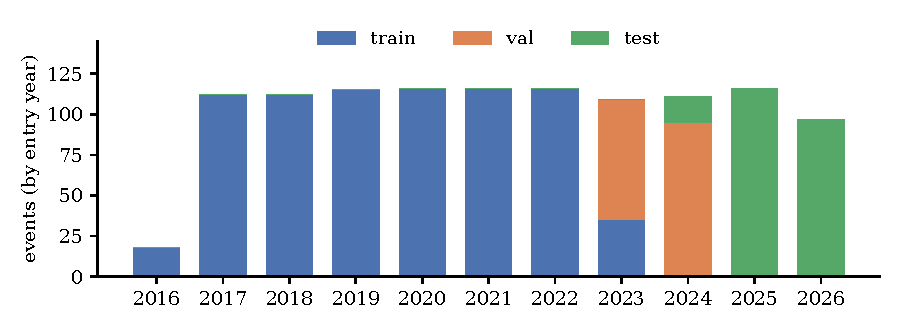
\includegraphics[width=0.9\linewidth]{generated/fig_coverage.pdf}
\caption{Events by entry year and split (document-only dataset, after purging).}
\label{fig:coverage}
\end{figure}

\section{Information timeline}\label{sec:timing}
All times are in America/New\_York. Let $A$ be the announcement time and $T$ the document time
(the EDGAR acceptance time).
\begin{itemize}
  \item \textbf{Session.} An event is BMO if $A$ is before 09:30, AMC if at or after 16:00, and DMH
  otherwise.
  \item \textbf{News cutoff.} Headlines count only if published before 00:00 ET on the date of~$A$, or
  before~$T$ if that is earlier. Provider timestamps are approximate, so same-day news is excluded
  rather than trusted.
  \item \textbf{Information date.} $D=\max(\mathrm{date}(A),\mathrm{date}(T))$.
  \item \textbf{Prediction and entry.} The prediction is made at 09:30 ET on the first trading day
  strictly after~$D$, and the position enters at that day's open. This deliberately skips a
  pre-open report's same-day open, because results may still be being discussed at 09:30.
  \item \textbf{Label.} The label is $\mathbf{1}[\mathrm{Close}_{x}/\mathrm{Open}_{e}>1]$, where $e$
  is the entry day and $x$ is the third trading session counting $e$ as the first. Trading days come
  from the price series, so holidays are handled.
\end{itemize}
Each of these is re-checked on the stored data: every headline timestamp is at or before the cutoff,
the entry is after the information date, and the label agrees with the stored return
(Figure~\ref{fig:timeline}). Because entry follows the announcement, the immediate price reaction is
already in the entry price. \emph{The label measures post-announcement drift.}

\begin{figure}[t]
\centering
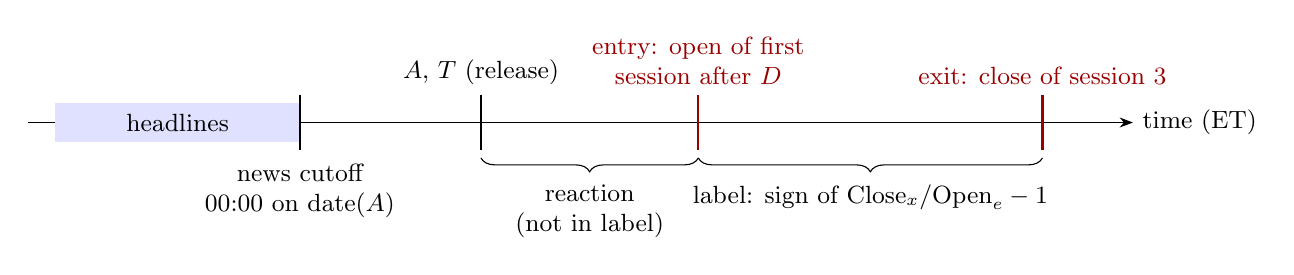
\begin{tikzpicture}[x=1.15cm,y=1cm,>=Stealth,font=\small]
  \draw[->] (0,0) -- (12.2,0) node[right] {time (ET)};
  \fill[blue!12] (0.3,-0.25) rectangle (3.0,0.25);
  \node at (1.65,0) {headlines};
  \draw[thick] (3.0,-0.35) -- (3.0,0.35);
  \node[below,align=center] at (3.0,-0.4) {news cutoff\\00:00 on date($A$)};
  \draw[thick] (5.0,-0.35) -- (5.0,0.35) node[above] {$A$, $T$ (release)};
  \draw[thick,red!60!black] (7.4,-0.35) -- (7.4,0.35) node[above,align=center] {entry: open of first\\ session after $D$};
  \draw[thick,red!60!black] (11.2,-0.35) -- (11.2,0.35) node[above] {exit: close of session 3};
  \draw[decorate,decoration={brace,mirror,amplitude=5pt}] (7.4,-0.45) -- (11.2,-0.45)
       node[midway,below=6pt] {label: sign of $\mathrm{Close}_x/\mathrm{Open}_e-1$};
  \draw[decorate,decoration={brace,mirror,amplitude=5pt}] (5.0,-0.45) -- (7.4,-0.45)
       node[midway,below=6pt,align=center] {reaction\\(not in label)};
\end{tikzpicture}
\caption{Information timeline for one event. Features use only text available before the entry
open; the label starts after the announcement reaction.}
\label{fig:timeline}
\end{figure}

\section{Model and baselines}\label{sec:model}
\paragraph{Encoder.} FinBERT is used frozen, pinned to a specific checkpoint revision. A document is
split into consecutive, non-overlapping 384-token chunks ($\le 8$ kept); each chunk is encoded and
mean-pooled over tokens, and chunk vectors are mean-pooled into one 768-dimensional document vector.
The pipeline also supports a second stream for headlines. When a stream is absent, its vector is
zeroed and a presence flag records the absence.
\paragraph{Fusion head.} The head concatenates the two vectors, their absolute difference, their
product and the presence flags, and applies dropout and either a single linear layer or one hidden
layer. It is trained with AdamW and early stopping on validation AUC. With one stream present, the
fused features reduce to the document vector and its magnitude.
\paragraph{Comparisons.} Every model sees only release text or less:
\begin{itemize}
  \item \textbf{Train-majority:} the training up-rate for every event.
  \item \textbf{Ticker prior:} each company's training up-rate, shrunk toward the global rate,
  $(\text{ups}+10\,\bar y)/(n+10)$. Every release names its company, so the embedding encodes identity.
  A text model that cannot beat this prior has not shown that the language matters.
  \item \textbf{Logistic regression} on the same frozen document features.
  \item \textbf{FinBERT fusion head.}
  \item \textbf{Zero-shot FinBERT:} the checkpoint's own sentiment classifier, scoring each of the
  first 8 chunks as $P(\text{positive})-P(\text{negative})$ and averaging. Nothing is trained.
\end{itemize}

\section{Protocol}\label{sec:protocol}
The protocol was written after the data were collected and before any model was trained on real
data, and was committed to version control. Its decisions are listed below.

Pre-registration here means the protocol was committed to version control before any real-data
training, and the selection file before the test stage. The public repository starts from a single
commit, so this order is documented in the protocol's change log and in the development-history
commit identifiers stored in the result files rather than in the public history; it was not lodged
with an external registry.
\begin{itemize}
  \item \textbf{Split.} Events are ordered by entry date and split chronologically at date
  boundaries (Table~\ref{tab:split}). Train events whose label windows reach into validation, and
  validation events reaching into test, are purged (\purgedTrain{} and \purgedVal{} events).
  \item \textbf{Selection.} On validation only:
  \begin{itemize}
    \item logistic regression over 1 or 8 chunks $\times$ $C\in\{0.01,0.1,1\}$;
    \item the fusion head over 1 or 8 chunks $\times$ 0 or 1 hidden layers, each with 5 seeds,
    choosing the best mean validation AUC.
  \end{itemize}
  The selected configurations were committed before the test stage, which refuses to run unless that
  file matches the committed version.
  \item \textbf{Test.} The test set was evaluated once.
  \item \textbf{Inference.}
  \begin{itemize}
    \item The primary metric is ROC AUC; AP, Brier score, log loss, accuracy and F1 are reported
    alongside it.
    \item Intervals come from \nBoot{} bootstrap resamples of whole entry weeks: events in the same
    week share market-wide moves.
    \item Model comparisons use paired differences on the same resamples.
  \end{itemize}
  \item \textbf{Claim rule, fixed in advance.} Release-language signal may be claimed only if a
  FinBERT model beats the ticker prior with a paired 95\% interval excluding zero.
\end{itemize}

\begin{table}[t]
\centering
\caption{Chronological split of the document-only dataset (after purging).}
\label{tab:split}
\begin{tabular}{lllrr}
\toprule
Split & First entry & Last entry & $n$ & Up-rate \\
\midrule
Train & 2016-10-19 & 2023-04-24 & 740 & 0.470 \\
Val & 2023-04-27 & 2024-10-24 & 169 & 0.527 \\
Test & 2024-10-31 & 2026-10-23 & 229 & 0.454 \\
\bottomrule
\end{tabular}

\end{table}

\section{Synthetic controls}\label{sec:controls}
Two synthetic datasets with the real schema and timeline bracket the pipeline. The ``documents'' are
built from stock sentences.
\begin{itemize}
  \item \textbf{Negative control.} Labels are drawn independently of the text, so any AUC far from 0.5
  would indicate leakage.
  \item \textbf{Positive control.} The text is bullish or bearish according to the label, and long
  enough to span several chunks, so a working pipeline must separate the classes.
\end{itemize}
With FinBERT and \ctlRuns{} seeds each (about \ctlTestN{} test events per seed), the negative control
scores a test AUC of \negMean{}~$\pm$~\negSd{} (range \negMin--\negMax), consistent with chance at this
sample size. The positive control scores \posMean{} on every seed (Table~\ref{tab:controls},
Figure~\ref{fig:controls}). These are pipeline checks, not market evidence.

\begin{table}[t]
\centering
\caption{Synthetic pipeline controls (FinBERT, seeds 0--4). Not market evidence.}
\label{tab:controls}
\begin{tabular}{lrcccc}
\toprule
Control & Runs & Head test AUC & Range & LR test AUC & Head val AUC \\
\midrule
Negative & 5 & 0.465 $\pm$ 0.075 & 0.392--0.578 & 0.469 & 0.548 \\
Positive & 5 & 1.000 $\pm$ 0.000 & 1.000--1.000 & 1.000 & 1.000 \\
\bottomrule
\end{tabular}

\end{table}

\begin{figure}[t]
\centering
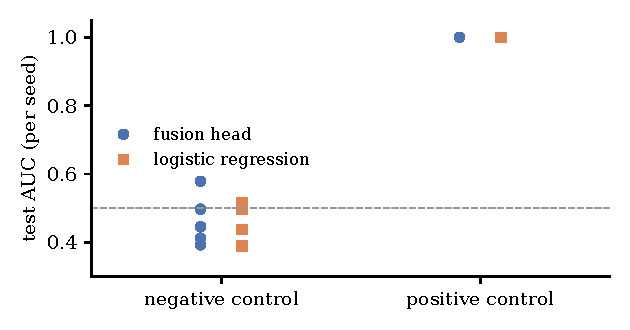
\includegraphics[width=0.6\linewidth]{generated/fig_controls.pdf}
\caption{Per-seed test AUC of the synthetic controls.}
\label{fig:controls}
\end{figure}

\section{Real-data results}\label{sec:results}
\paragraph{Selection (validation).} Table~\ref{tab:grid} shows the validation grid. Logistic regression
was selected with \selLRChunks{} chunk and $C=\selLRC$; the fusion head with \selHeadChunks{} chunk and
\selHeadLayers{} hidden layers (mean validation AUC \valHeadSelect{}). Configurations using 8 chunks
did not do better on validation.

\begin{table}[t]
\centering
\caption{Validation grid used for selection (validation data only). Fusion-head values are mean $\pm$
s.d.\ over 5 seeds; each seed's value is at its early-stopping epoch.}
\label{tab:grid}
\begin{tabular}{llrr}
\toprule
Model & Setting & Chunks & Val AUC \\
\midrule
Logistic regression & $C=0.01$ & 1 & 0.539 \\
Logistic regression & $C=0.1$ & 1 & 0.523 \\
Logistic regression & $C=1$ & 1 & 0.524 \\
Logistic regression & $C=0.01$ & 8 & 0.498 \\
Logistic regression & $C=0.1$ & 8 & 0.453 \\
Logistic regression & $C=1$ & 8 & 0.452 \\
\midrule
Fusion head & 0 hidden layers & 1 & 0.602 $\pm$ 0.008 \\
Fusion head & 1 hidden layer & 1 & 0.594 $\pm$ 0.005 \\
Fusion head & 0 hidden layers & 8 & 0.568 $\pm$ 0.010 \\
Fusion head & 1 hidden layer & 8 & 0.579 $\pm$ 0.007 \\
\bottomrule
\end{tabular}

\end{table}

\paragraph{Held-out test.} On \nTest{} test events in \nWeeks{} entry weeks
(\firstTest{} to \lastTest), no model is distinguishable from chance (Table~\ref{tab:test},
Figure~\ref{fig:auc}).
\begin{itemize}
  \item The fusion head reaches \testHead{} (\loHead--\hiHead); its seeds range \headSeedMin--\headSeedMax.
  \item Logistic regression reaches \testLR{}, zero-shot FinBERT \testZs{} and the ticker prior \testTick.
  \item The paired difference between the fusion head and the ticker prior is \diffHeadTick{}
  (\diffHeadTickLo{} to \diffHeadTickHi{}; Table~\ref{tab:diff}). By the pre-registered rule, no
  release-language signal is claimed.
  \item On probability quality, the fusion head's Brier score (\brierHead) and log loss (\loglossHead)
  are no better than the train-majority's (\brierMaj, \loglossMaj).
\end{itemize}

\begin{table}[t]
\centering
\caption{Held-out test results (evaluated once). Intervals: 95\% week-block bootstrap. Zero-shot
FinBERT produces rank-only scores, so probability metrics are not reported for it.}
\label{tab:test}
\resizebox{\linewidth}{!}{\begin{tabular}{lrrcrrrrr}
\toprule
Model & Val AUC & Test AUC & 95\% CI & AP & Brier & Log loss & Acc. & F1 \\
\midrule
Train-majority & 0.500 & 0.500 & [0.500, 0.500] & 0.454 & 0.248 & 0.689 & 0.546 & 0.000 \\
Ticker prior & 0.566 & 0.487 & [0.423, 0.556] & 0.448 & 0.258 & 0.710 & 0.528 & 0.407 \\
Logistic regression & 0.539 & 0.461 & [0.383, 0.538] & 0.456 & 0.293 & 0.786 & 0.450 & 0.515 \\
FinBERT fusion head & 0.601 & 0.506 & [0.439, 0.573] & 0.455 & 0.259 & 0.711 & 0.463 & 0.580 \\
Zero-shot FinBERT & 0.532 & 0.469 & [0.388, 0.552] & 0.434 & -- & -- & -- & -- \\
\bottomrule
\end{tabular}
}
\end{table}

\begin{table}[t]
\centering
\caption{Paired test-AUC differences on the same week-block resamples, with the share of resamples in
which the difference is $\le 0$.}
\label{tab:diff}
\begin{tabular}{lrcr}
\toprule
Test AUC difference & Estimate & 95\% CI & Share $\le 0$ \\
\midrule
FinBERT fusion head $-$ Ticker prior & $+$0.019 & [$-$0.052, $+$0.089] & 0.31 \\
Logistic regression $-$ Ticker prior & $-$0.026 & [$-$0.111, $+$0.052] & 0.73 \\
Zero-shot FinBERT $-$ Ticker prior & $-$0.018 & [$-$0.119, $+$0.081] & 0.66 \\
FinBERT fusion head $-$ Logistic regression & $+$0.045 & [$-$0.042, $+$0.129] & 0.16 \\
Ticker prior $-$ Train-majority & $-$0.013 & [$-$0.077, $+$0.056] & 0.64 \\
\bottomrule
\end{tabular}

\end{table}

\begin{figure}[t]
\centering
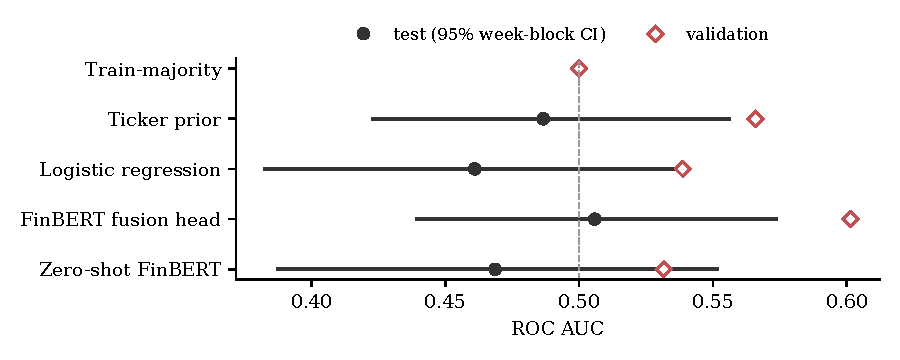
\includegraphics[width=0.9\linewidth]{generated/fig_test_auc.pdf}
\caption{Validation AUC (open diamonds) and held-out test AUC with 95\% week-block intervals.}
\label{fig:auc}
\end{figure}

\paragraph{Validation optimism.} Validation AUCs of \valZs--\valHead{} did not carry over to test, for two
identifiable reasons:
\begin{itemize}
  \item The fusion head's validation number is optimistic by construction, because each seed is
  stopped at its best validation epoch.
  \item The ticker prior also fell from \valTick{} on validation to \testTick{} on test: the companies
  that had tended to rise after earnings changed between periods.
\end{itemize}
Selecting on the validation set and evaluating once on a later test set is designed to expose exactly
this kind of gap.

\paragraph{Exploratory: headlines.}\label{sec:explore} Labelled exploratory; nothing was trained or
selected. On the \explN{} events that have pre-cutoff headlines (\explWeeks{} entry weeks), zero-shot
FinBERT sentiment of the headlines has an AUC of \explAuc{} (\explLo--\explHi). On the \explBothN{} of
those events that also have a release, release sentiment scores \explDocAuc{}, and the difference is
\explDiff{} (\explDiffLo{} to \explDiffHi). Neither score distinguishes direction from chance in this
small sample.

\section{Limitations and threats to validity}
\begin{itemize}
  \item \textbf{Target.} The label is three-session drift after the entry open, not the announcement
  reaction, which is already priced in for these companies. The result says nothing about whether
  release text explains the reaction.
  \item \textbf{Precision.} The test interval half-width is about \halfWidthHead{} AUC. Effects smaller
  than that cannot be detected here.
  \item \textbf{Text coverage.} Only the first ${\sim}380$ tokens (selected) or ${\sim}3$k tokens of
  releases with a median of \tokMedian{} tokens are encoded. Call transcripts, analyst Q\&A and
  expectations (the surprise) are not used, and the encoder is not fine-tuned.
  \item \textbf{Universe.} The universe is today's large capitalisation names projected back to 2016,
  which introduces survivorship bias. ExxonMobil is effectively absent and Disney is missing before
  2019. Results may differ for smaller, less-covered firms.
  \item \textbf{Timing data.} Yahoo announcement times are approximate. The conservative cutoff and the
  entry rule make the label insensitive to the stamped minute, at the cost of excluding same-day news.
  \item \textbf{Identity.} Releases name their company, so embeddings encode identity. The ticker prior
  controls for this, but only for stable company effects.
  \item \textbf{Reproduction.} The frozen datasets contain provider data and are not redistributed. A
  fresh collection with the same code yields a similar but not identical dataset, because provider data
  change. The code, fingerprints, manifests and all result files are public.
  \item \textbf{Not trading performance.} Classification metrics are not trading returns, and nothing
  here supports a trading claim.
\end{itemize}

\section{Reproducibility}
The repository contains the code, tests, dependency lock, pre-registered protocol, run manifests and
the result files from which every number, table and figure in this paper is generated by
a script (\path{experiments/paper_assets.py}). The real-data steps are:
{\small
\begin{verbatim}
python main.py --data-mode real --collect-only   # collection + coverage
python experiments/phase4.py select              # validation only
python experiments/phase4.py test                # needs committed selection
python experiments/phase4.py headlines           # exploratory
python experiments/paper_assets.py               # numbers, tables, figures
python main.py --data-mode synthetic-positive-control   # no credentials
\end{verbatim}}
The synthetic controls need no credentials. Real collection needs a contact
User-Agent for SEC EDGAR and, for headlines, a Finnhub key, both supplied through environment
variables.

\bibliographystyle{plainnat}
\bibliography{references}

\end{document}
